% gsw-eval final report. DRAFT written with an AI assistant: the team must check every claim
% and rewrite the text in their own words before submission (see the AI-use statement).
% Every number in the tables comes from results/ via `gsw-eval report`; never type numbers by hand.
\documentclass[11pt]{article}
\usepackage[final]{acl}
\usepackage{times}
\usepackage{latexsym}
\usepackage[T1]{fontenc}
\usepackage[utf8]{inputenc}
\usepackage{microtype}
\usepackage{inconsolata}
\usepackage{graphicx}
\usepackage{booktabs}
\usepackage{xcolor}

% Visible markers for what is still missing. Remove all before submission.
\newcommand{\todo}[1]{\textcolor{red}{\textbf{[TODO: #1]}}}

\title{What Does Swiss German Cost a Language Model?\\
Separating Dialect from Spelling in LLM Normalization}

\author{Erik Avtandilyan \and Simone Martinecz \and Kelvin Myers \\
  University of Zurich \\
  Essentials in Text and Speech Processing, HS 2026 \\
  \texttt{https://github.com/Eroavt/gsw-eval}}

\begin{document}
\maketitle

\begin{abstract}
Swiss German is spoken by about five million people but has no standard spelling, so every
writer spells it their own way. Large language models (LLMs) understand it worse than Standard
German and need more tokens for it. We ask how much of this cost comes from the dialect and how
much from the spelling. We build \textsc{gsw-eval}, an open, reproducible benchmark that feeds
the same 500 sentences to a model as Standard German, as careful Swiss German in eight dialects,
and as texting-style and character-noised Swiss German. On SwissDial, the dialect costs
Apertus~8B 20.1 chrF points and Llama~3.1~8B 24.4 points; texting spelling adds only 3.4 and 4.9.
The Swiss model Apertus beats Llama by 7.1 points, and the gap grows under noisy spelling.
Token counts tell the same story: Swiss German needs 16 to 30\% more tokens than Standard German,
while texting spelling changes the count by about 1\%. Per-dialect difficulty follows how close
each written dialect is to Standard German ($r = 0.93$). \todo{one sentence on the fresh set and
the human ratings once they are in.}
\end{abstract}

\section{Introduction}

Written Swiss German is everywhere in Switzerland: in messages, social media and comments.
It is also a textbook case of a low-resource variety inside a high-resource language: Standard
German is one of the best-served languages in NLP, its dialects are not \citep{joshi2020state}.
Two things make Swiss German hard for a language model. First, the \emph{dialect}: the eight
major dialects differ in vocabulary, sound and grammar. Second, the \emph{spelling}: there is
no orthography, so the same writer may spell a word differently from one message to the next.

Users pay for both, in quality and in money, since API prices are per token and non-standard
text splits into more tokens \citep{petrov2023unfairness,ahia2023cost}. But the two causes need
different fixes. A dialect problem calls for more dialect data; a spelling problem could be
solved with normalization or with robust training. Existing work measures one or the other.
We measure both on the same sentences.

\paragraph{Contributions.}
\begin{enumerate}
\itemsep0em
\item \textsc{gsw-eval}, an open benchmark that runs any LLM on written Swiss German and splits
the quality loss into a \emph{dialect cost} and a \emph{spelling cost}, with confidence intervals.
\item A comparison of a Swiss and a non-Swiss model of the same size, plus a commercial reference,
showing that \todo{headline finding, final wording after the Claude run}.
\item A token-tax analysis of nine tokenizers, showing that the extra tokens come from the
dialect, not from the spelling.
\item A small fresh test set in which each native writer translates the same sentences twice,
carefully and in texting style. \todo{size once collected}
\end{enumerate}

\section{Related Work}
\todo{Kelvin: rewrite this section in your own words, 0.5 column.}

\textbf{Swiss German NLP.} Earlier work normalizes Swiss German transcripts to a common spelling
with character-level machine translation \citep{scherrer2016normalisation} on the ArchiMob
corpus \citep{samardzic2016archimob}. SwissBERT \citep{vamvas2023swissbert} adapts an encoder to
Swiss national languages, and \citet{vamvas2024modular} adapt encoders to written Swiss German.
SwissDial \citep{dogan2021swissdial} provides the same sentences in eight dialects with Standard
German references, which makes a controlled comparison across dialects possible. Collecting
dialect data remains the bottleneck \citep{sun2025dialingle}.

\textbf{Dialect and noise robustness.} DialectBench \citep{faisal2024dialectbench} shows large
gaps between standard and non-standard varieties across many tasks. Synthetic character noise
breaks neural translation \citep{belinkov2018noise}, and injecting such noise during training
helps transfer between closely related languages \citep{aepli2022noise}. We use the same noise
for evaluation and compare it with rule-based texting spelling.

\textbf{Tokenization cost.} The same content needs very different numbers of tokens in
different languages \citep{rust2021tokenizer,petrov2023unfairness}, which makes commercial models
more expensive for some users \citep{ahia2023cost}. We apply this lens \emph{within} one
language: Standard German versus its dialects.

\section{Data}
\label{sec:data}

\textbf{SwissDial.} SwissDial v1.1 \citep{dogan2021swissdial} contains 11,213 Standard German
sentences with transcriptions in up to eight dialects (AG, BE, BS, GR, LU, SG, VS, ZH), one
writer per dialect. We keep the 2,529 sentences available in all eight dialects and drop 232
marked as code-switching, leaving 2,297. We draw a fixed split of 50 development and 500 test
sentences (seed 13), giving 4,000 Swiss German test inputs per condition. The Standard German
sentence is always the reference.

\textbf{Fresh set.} \todo{Simone: who wrote it (number of writers, dialects), how long it took.}
Each writer translated the same 30 Standard German sentences (20 everyday chat, 10 news-like)
twice: once carefully and once ``the way you would text''. Because the same person writes both
versions, the difference between them is spelling only. The set was written after the models
were trained, so it cannot be in their training data. It is released with the code (CC BY 4.0).

\section{Method}

\textbf{Conditions.} Every test sentence is given to each model in four forms:
(1)~\emph{Standard German input}: the reference itself;
(2)~\emph{clean}: the SwissDial transcription;
(3)~\emph{texting}: the clean text rewritten by 24 texting rules (lower case, dropped
punctuation, collapsed double vowels, short forms such as \emph{vlt} for \emph{vilicht}),
each firing with a probability, \todo{Simone: confirm the rules are realistic}; and
(4)~\emph{character noise}: 10\% of words get one random letter insertion, deletion or
substitution, following \citet{aepli2022noise}. All noise is seeded per sentence.

\textbf{Baselines.} The \emph{identity} baseline copies the Swiss German input unchanged; it is
the lower bound every model must beat. The \emph{Standard German input} condition is the upper
bound: the best a model can do when there is no dialect and no spelling problem.

\textbf{Dialect and spelling cost.} We define the \emph{dialect cost} as chrF on Standard German
input minus chrF on clean Swiss German, and the \emph{spelling cost} as chrF on clean minus chrF
on texting input. Both are computed on the same sentences, so content is held constant.

\textbf{Models.} Apertus 8B Instruct \citep{apertus2025}, trained with a strong Swiss and
multilingual focus, and Llama 3.1 8B Instruct \citep{grattafiori2024llama3}, the same size
without a Swiss focus, both run locally with 8-bit weights and greedy decoding via MLX. Claude
Sonnet 5.5 serves as a commercial reference. \todo{Claude results.} All models receive the same
German prompt asking for the Standard German sentence only.

\textbf{Metric and statistics.} We score with chrF \citep{popovic2015chrf} as implemented in
sacreBLEU \citep{post2018sacrebleu}; character n-grams suit a task where most errors are partial
word forms. All intervals are 95\% bootstrap intervals over sentences \citep{koehn2004significance};
model differences use a paired bootstrap, and the costs use a cluster bootstrap that resamples
whole sentences with all their dialects. We remove answer preambles such as ``Der Satz lautet
auf Standarddeutsch:'', which 4.5\% of 8B outputs contain.

\textbf{Token tax.} For a tokenizer, the token tax is the number of tokens of the Swiss German
sentences divided by the tokens of the same sentences in Standard German, summed over all 2,297
parallel sentences and eight dialects. Because the texting rules drop punctuation and punctuation
marks are tokens, we compare all conditions with punctuation removed.

\textbf{Human evaluation.} \todo{Kelvin + Simone: two native speakers rated 96 outputs (48 inputs
x 2 models, blind, random order) for adequacy on a 1--5 scale; report kappa here.}

\section{Results}

\begin{table*}[t]
\centering
\begin{tabular}{lrrrrrr}
\toprule
Model & Std.\ German & Clean & Texting & Char.\ noise & Dialect cost & Spelling cost \\
\midrule
Identity (lower bound) & 100.0\,{\scriptsize$\pm$0.0} & 46.9\,{\scriptsize$\pm$1.0} & 40.0\,{\scriptsize$\pm$0.8} & 45.3\,{\scriptsize$\pm$1.0} & 53.1\,{\scriptsize$\pm$1.0} & 6.8\,{\scriptsize$\pm$0.4} \\
Apertus 8B & 94.0\,{\scriptsize$\pm$1.0} & 74.1\,{\scriptsize$\pm$1.2} & 70.6\,{\scriptsize$\pm$1.2} & 71.3\,{\scriptsize$\pm$1.1} & 19.9\,{\scriptsize$\pm$1.2} & 3.5\,{\scriptsize$\pm$0.5} \\
Llama 3.1 8B & 91.5\,{\scriptsize$\pm$1.0} & 67.7\,{\scriptsize$\pm$1.2} & 62.7\,{\scriptsize$\pm$1.3} & 64.8\,{\scriptsize$\pm$1.2} & 23.8\,{\scriptsize$\pm$1.2} & 5.0\,{\scriptsize$\pm$0.6} \\
Gemma 3 27B & 84.7\,{\scriptsize$\pm$1.1} & 75.2\,{\scriptsize$\pm$1.1} & 72.6\,{\scriptsize$\pm$1.1} & 73.3\,{\scriptsize$\pm$1.1} & 9.4\,{\scriptsize$\pm$1.2} & 2.6\,{\scriptsize$\pm$0.5} \\
Claude Sonnet 5.5 & 94.2\,{\scriptsize$\pm$1.0} & 85.6\,{\scriptsize$\pm$0.9} & 84.5\,{\scriptsize$\pm$0.9} & 84.2\,{\scriptsize$\pm$0.9} & 8.6\,{\scriptsize$\pm$1.1} & 1.1\,{\scriptsize$\pm$0.3} \\
\bottomrule
\end{tabular}

\caption{chrF on the 500 test sentences ($\pm$: half-width of the 95\% bootstrap interval). Swiss
German columns pool 4,000 inputs over eight dialects. Dialect cost = Standard German input minus
clean; spelling cost = clean minus texting.}
\label{tab:quality}
\end{table*}

\textbf{The dialect costs far more than the spelling.} Table~\ref{tab:quality} shows that moving
from Standard German to clean Swiss German costs Apertus 20.1 and Llama 24.4 chrF points. Texting
spelling costs a further 3.4 and 4.9 points, and character noise 2.8 and 3.0. Both models stay far
above the identity baseline (46.7), so they do translate rather than copy.

\textbf{The Swiss model is better, and more robust.} Apertus beats Llama in every condition
(paired bootstrap, $p < 0.001$): by 2.8 points on Standard German input, 7.1 on clean dialect and
8.6 on texting input. The advantage is largest where the input is least standard, which suggests
that exposure to Swiss text helps most where spelling varies.

\textbf{Even Standard German is not copied.} Neither model reaches 100 on Standard German input:
Apertus returns the sentence unchanged 64\% of the time, Llama only 45\%; the rest are
paraphrases such as ``Jemand stört mich hier bei meiner Arbeit'' for ``Irgendjemand pfuscht mir
hier ins Handwerk''. This is why the upper bound matters: part of every model's gap to 100 is
paraphrase that chrF counts as error, not misunderstanding. \todo{the human ratings tell how big
this part is.}

\begin{figure}[t]
\centering
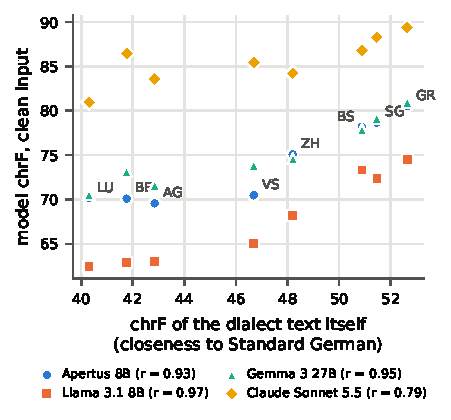
\includegraphics[width=\columnwidth]{../results/figures/dialects.pdf}
\caption{Per-dialect chrF of each model (clean input) against the chrF of the untranslated
dialect text, a measure of how close its spelling is to Standard German.}
\label{fig:dialects}
\end{figure}

\textbf{Hard dialects are the ones written farthest from Standard German.} Scores range from
69.0 (AG) to 80.0 (GR) for Apertus, and the ranking is almost the same for Llama
(Figure~\ref{fig:dialects}). Both correlate strongly with the identity score of each dialect
($r = 0.93$ and $0.94$): models do worst where the written form is farthest from Standard German.
Since SwissDial has one writer per dialect, this mixes the dialect with the writer's personal
spelling. The fresh set separates the two. \todo{fresh-set result.}

\begin{table}[t]
\centering
\small
\begin{tabular}{lrrrr}
\toprule
Tokenizer & Tok./word & Tax & Range & Texting \\
\midrule
Apertus 8B & 1.64 & 1.18 & 1.12--1.27 & +0.3\% \\
Llama 3.1 8B & 1.93 & 1.08 & 1.03--1.15 & -1.3\% \\
Gemma 3 & 1.62 & 1.13 & 1.09--1.22 & +0.0\% \\
Qwen 3 & 1.92 & 1.08 & 1.04--1.16 & -1.0\% \\
Mistral 7B v0.3 & 2.10 & 1.07 & 1.03--1.14 & -0.7\% \\
OpenAI o200k & 1.60 & 1.15 & 1.12--1.24 & -0.4\% \\
XLM-R & 1.63 & 1.18 & 1.13--1.26 & +0.8\% \\
SwissBERT & 1.43 & 1.42 & 1.32--1.52 & +7.1\% \\
\bottomrule
\end{tabular}

\caption{Token tax per tokenizer. Tok./word: tokens per word of Standard German. Tax: tokens
for Swiss German divided by tokens for the same Standard German sentences (punctuation removed,
eight dialects pooled). Range: cheapest to most expensive dialect. Texting: change of the tax
caused by texting spelling.}
\label{tab:tax}
\end{table}

\textbf{Token tax comes from the dialect, not the spelling.} Swiss German needs 16\% (Mistral) to
30\% (Apertus, XLM-R) more tokens than the same content in Standard German
(Table~\ref{tab:tax}). Texting spelling changes this by about 1\% for every LLM tokenizer: it
creates rarer word forms but also shortens words, and the two effects cancel. Bernese is the most
expensive dialect and Zurich German the cheapest for all LLM tokenizers. Apertus pays the highest
\emph{relative} tax only because its tokenizer is very efficient on Standard German
(1.64 tokens per word against 1.93 for Llama); in absolute terms it needs fewer tokens for Swiss
German than Llama. \todo{price per 1,000 sentences for Claude once the key is set.}

\textbf{Robustness.} \todo{prompt check (3 prompts) and full precision vs 8-bit, from the MacBook
Pro runs: does the ranking change?}

\textbf{Human ratings.} \todo{kappa, Spearman chrF vs rating, and whether chrF picks the same
better model as the raters.}

\textbf{Fresh set.} \todo{real vs synthetic texting cost, per writer.}

\section{Discussion and Limitations}

\todo{Kelvin + Erik: write after all results are in. Points to cover:}
(1)~SwissDial transcriptions are free translations by one writer per dialect, so dialect and
writer are confounded; the fresh set addresses this only for \todo{N} writers.
(2)~The texting rules are hand-written and applied with fixed probabilities; real texting is
richer (abbreviations, emoji, code-switching).
(3)~chrF punishes valid paraphrases; the human ratings estimate how much.
(4)~We test one prompt per model in the main run and 8-bit weights; the robustness checks cover
both on a subset.
(5)~SwissDial has been public since 2021 and may be in the models' training data; the fresh set
cannot be.

\section{Conclusion}
\todo{3--4 sentences: answer the question in the title with the two numbers.}

\section*{Code and Data}
Code, outputs of every model, and the fresh set: \url{https://github.com/Eroavt/gsw-eval}.
Every number in this report can be reproduced with one command, \texttt{scripts/reproduce.sh},
which needs neither a GPU nor an API key because all model outputs are cached.

\section*{Use of AI Assistants}
We used an AI coding assistant (Claude Code) to write and test the code and to draft parts of
this report. All design decisions, the data collection and the final text are our own, and we
checked every number against the code's output. \todo{adapt to UZH rules.}

\bibliography{refs}

\end{document}
